\documentclass[20pt,landscape]{foils}
\usepackage{mbtslides}
\usepackage[english]{babel}
\usepackage{graphicx}
\usepackage{marvosym}
\usepackage{amssymb}  % provides \gtrsim
\usepackage{ellipse}
\usepackage{fancyvrb}
\usepackage{ulem}  % provides \sout
\usepackage[cm]{sfmath}

% This is supposed to make underscores cut'n'pastable
% Not sure what the lmodern package does or whether it's needed for this.
% But it's not working (though apparently it did in nam2023)
% \usepackage[T1]{fontenc}
% \usepackage{lmodern}
% \usepackage{textcomp}
% \DeclareTextSymbolDefault{\textunderscore}{T1}

\setlength{\unitlength}{1cm}


\newcommand{\bhref}[2]{\href{#1}{{\color{blue}#2}}}
\newcommand{\burl}[1]{{\color{blue}\url{#1}}}
\newcommand{\rfc}[1]{\bhref{https://www.rfc-editor.org/rfc/rfc#1}
                           {RFC\,#1}}

\newcommand{\buttimg}[1]
           {\mbox{\vtop{\vskip-2ex\hbox{\includegraphics[height=3ex]{#1}}}}}
\newcommand{\tcicon}[1]{
   \mbox{\vtop{\vskip-2.5ex\hbox{\includegraphics[height=3ex]{#1}}}}}
\newcommand{\buttitem}[1]{\item[{\makebox[0cm][r]{\tcicon{#1}}}]}
\definecolor{darkergreen}{rgb}{0,0.38,0}
\definecolor{purple}{rgb}{0.8,0,0.8}

% Fixes problem with includegraphics images screwing up colours on their
% page in the output PDF.  I have no idea *how* it fixes it mind.
\pdfpageattr {/Group << /S /Transparency /I true /CS /DeviceRGB>>}

% Oh no, this is required on my Ubuntu 22.04 (though not 20.04) installation
% to make the \ellipse commands work.
\makeatletter
\newdimen\@tempdimd
\makeatother

\begin{document}
\sf

\newcommand{\bigword}[1]{
  \vspace*{7cm}
  \begin{center}
    \color{darkblue}
    \scalebox{3}{
      \Huge\bf #1
    }
  \end{center}
  \addtocounter{page}{-1}
}

\rightfooter{}
\MyLogo{}

\vspace*{3cm}
\hspace*{5cm}
\begin{minipage}{30cm}
\LARGE
\begin{enumerate}
  \item Wins
  \item Issues
  \item Matching with TOPCAT and STILTS
  \item AOB
\end{enumerate}
\end{minipage}

\newpage
\bigword{Wins?}
\newpage
\bigword{Issues?}
\newpage

\MyLogo{\color{grey}
        Mark Taylor, Crossmatching with TOPCAT and STILTS
        Bristol Astro Dev Group,
        17 January 2025}
\rightfooter{\quad{\color{grey}\thepage/\pageref*{lastPage}}}
\setcounter{page}{1}

\vspace*{1.0cm}
\begin{center}
{\color{darkblue}
\framebox{\Huge\bf
  \begin{minipage}{0cm}
  \begin{tabbing}
  Crossmatching with \\
  TOPCAT and STILTS
  \end{tabbing}
  \end{minipage}
}}
\\[2.0cm]
{\Large 
  Mark Taylor
}
\\[2.0cm]
{\large\color{grey}
  Bristol Astro Dev Group
  \\[2ex]
  17 January 2024
}
\end{center}

\vspace*{1.5cm}
\begin{center}
  \tiny
  \color{brown}
  \input gitid
\end{center}

% \slide{Summary}

\slide{Matching}

\begin{list0}
  \item Typical science question:
  \begin{list2big}
    \item[] {\color{darkred}\sl
             Which sources from one observation correspond to
             which sources from another observation?}
  \end{list2big}
  \item Basic mathematical question:
  \begin{list2big}
    \item[] {\color{darkred}\sl
             Which positions in a list are close to
             which positions in another list?
             (for some definition of ``close to'')}
  \end{list2big}
  \item Conceptually straightforward ...
  \begin{list2big}
    \item for each position in one list, test each position in the other list
    \item write it yourself?
  \end{list2big}
  \item ... but there are complications
% \begin{list2big}
%   \item maybe use existing software
% \end{list2big}
\end{list0}

\newcommand{\matchfigSlide}[1]{
  \slide{Matching}
  \vspace*{0.5cm}
  \begin{center}
    \includegraphics[height=16cm]{#1}
  \end{center}
}
\matchfigSlide{match1.pdf}
\matchfigSlide{match2.pdf}
\addtocounter{page}{-1}
\matchfigSlide{match3.pdf}
\addtocounter{page}{-1}
\matchfigSlide{match4.pdf}
\addtocounter{page}{-1}

\slide{Complications}

\begin{list1}
\vspace*{-0.2cm}
  \item Resource Usage
\vspace*{-0.2cm}
  \begin{list2}
    \item Algorithms that work nicely for 100 objects might be
          (much) too slow for 1,000,000 objects
\vspace*{-0.1cm}
    \item Memory usage can be an issue
  \end{list2}
\vspace*{-0.2cm}
  \item Spherical geometry
\vspace*{-0.2cm}
  \begin{list2}
    \item Careful when calculating distances for nearby objects (numerics)
\vspace*{-0.1cm}
    \item Careful near the antimeridian
\vspace*{-0.1cm}
    \item Careful near the poles
\vspace*{-0.1cm}
    \item How to chop the sky up into boxes?
  \end{list2}
\vspace*{-0.2cm}
  \item Other geometries
\vspace*{-0.2cm}
  \begin{list2}
    \item N-dimensional Cartesian spaces
\vspace*{-0.1cm}
    \item Sky + N-dimensional Cartesian spaces
  \end{list2}
\vspace*{-0.2cm}
  \item Different match criteria
\vspace*{-0.2cm}
  \begin{list2}
    \item Per-object error radius
\vspace*{-0.1cm}
    \item Elliptical/anisotropic match radius
  \end{list2}
\vspace*{-0.2cm}
  \item Related questions
\vspace*{-0.2cm}
  \begin{list2}
    \item Which objects {\sl don't\/} have any matches?
  \end{list2}
\vspace*{-0.2cm}
  \item Correctness
\vspace*{-0.2cm}
  \begin{list2}
    \item Are you sure you've got the right answer?
  \end{list2}
\end{list1}


\newcommand{\tcslide}[1]{
  \newpage
  \begin{picture}(32,0)
  \put(0,-19){
\includegraphics[height=19cm]{tclogo.pdf}}
  \put(21,-9){\begin{minipage}{16cm} #1 \end{minipage}}
  \end{picture}
}

\tcslide{}
\tcslide{
  \begin{list0}
    \item Get TOPCAT to do it for you!
    \begin{list2big}
      \item Internal match functionality
      \item Talk to match-capable external services
    \end{list2big}
  \end{list0}
}
\addtocounter{page}{-1}

\slide{TOPCAT Internal Matching Function}

\begin{picture}(30,0)
\put(23,-17){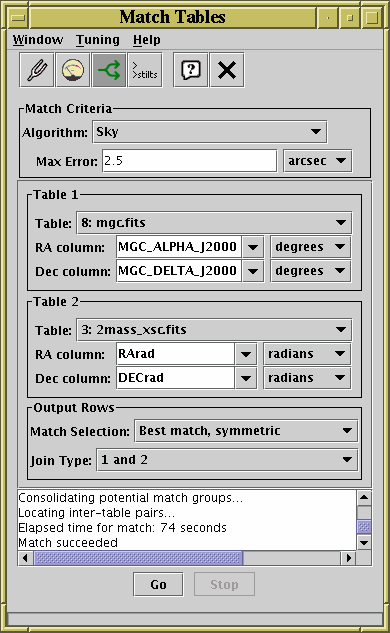
\includegraphics[height=17cm]{MatchWindow.png}}
\end{picture}
\vspace*{-1.5cm}

\begin{list0}
  \item TOPCAT can match tables you've loaded into it
  \begin{list2big}
    \item Use \buttimg{matchTwo2.png} {\bf Pair Match} window
    \begin{list3}
      \item (other windows in {\bf Joins} menu for
             matching 1 or 3, 4, 5, ... tables)
    \end{list3}
    \item Select match type, input tables etc and hit {\bf Go}
    \item Result is usually a new matched table
  \end{list2big}
  \item Works well up to $\sim$ 10 million rows
  \begin{list3}
    \item though you can push it further with time and memory
  \end{list3}
  \item Pretty fast ($\lesssim$ couple of minutes)
  \item Quite flexible
  \begin{list3}
    \item sky, Cartesian, exact, 3D, ellipses, errors, combinations, ...
  \end{list3}
\end{list0}

\slide{TOPCAT for External Match Services}

\begin{picture}(30,0)
\put(24,-17){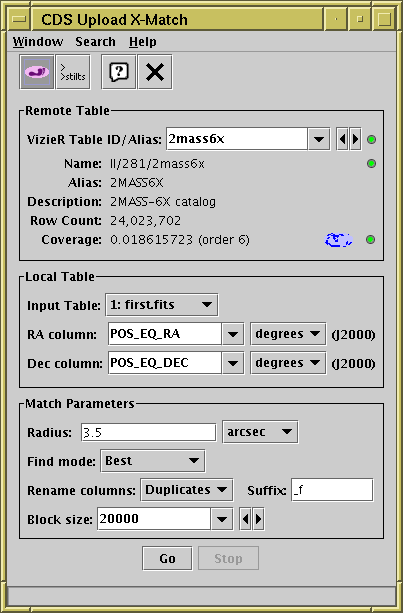
\includegraphics[height=17cm]{CdsUploadMatchWindow.png}}
\end{picture}
\vspace*{-1.5cm}

\begin{list0}
  \item TOPCAT can send a table you've loaded to a match service
  \item Usually best: {\bf CDS X-Match Service}
  \begin{list2big}
    \item Use \buttimg{xm3.png} {\bf CDS X-Match Upload} window
    \item Fill in remote (VizieR) table
    \begin{list3}
      \item Select from menu, or use
            \bhref{https://vizier.cds.unistra.fr/}{VizieR web page}
            to find ID
    \end{list3}
    \item Fill in local table, match criteria etc, hit {\bf Go}
    \item No size limit (TOPCAT chops up query into chunks for you)
    \item Usually pretty fast
    \begin{list2big}
      \item[] ... but sometimes slow or broken.
              Complain to \bhref{mailto:cds-question@unistra.fr}{CDS} or me.
    \end{list2big}
    \item May not have all the columns you want
  \end{list2big}
  \item Other options:
  \begin{list2big}
    \item TAP upload query (flexible, harder to use)
    \item Multi-cone search (slow, not generally recommended)
  \end{list2big}
  \item Works for external tables too large to load (e.g.\ large surveys)
  \item Result is a new matched table
\end{list0}

\slide{STILTS}

\vspace*{-0.2cm}
\begin{list0}
  \item STILTS is a set of command-line tools
  \begin{list2big}
    \item Does more or less all the same things as TOPCAT, but scriptably
    \item In some cases more scalable than TOPCAT
          (but generally not for matching commands)
    \item Can run it like:\\
          \hspace*{3em}
          {\color{brown}\verb|stilts <subcommand> arg=value arg=value ...|} \\
          or maybe: \\
          \hspace*{3em}
          {\color{brown}\verb|topcat -stilts <subcommand> arg=value arg=value ...|}
    \item Lots of documentation at
          \burl{http://www.starlink.ac.uk/stilts/sun256/}
  \end{list2big}
  \item STILTS matching commands:
  \begin{list2}
    \item[] {\color{brown}\tt tmatch2}: match 2 tables locally
    \item[] {\color{brown}\tt tmatch1}: match within 1 table locally
    \item[] {\color{brown}\tt cdsskymatch}: match local table with remote one
                                            using CDS X-Match service
    \item[] {\color{brown}\tt tapskymatch}: match local table with remote one
                                            using TAP service
    \item[] \hspace*{2em} ... etc
  \end{list2}
\vspace*{-0.2cm}
  \item Example: \\
\vspace*{-0.2cm}
        {\color{brown}\small
        \begin{verbatim}
    stilts tmatch2 in1=obs_v.xml in2=obs_i.xml out=obs_iv.xml \
                   matcher=sky values1="ra dec" values2="ra dec" params="2"
        \end{verbatim}}
\end{list0}

\slide{TOPCAT/STILTS Interoperability}


\slide{TOPCAT/STILTS Matching Limitations}

\begin{list0}
  \item Scalability
  \begin{list2}
    \item TOPCAT internal matching doesn't work so well for large catalogues
    \begin{list3}
      \item $N \lesssim 10^{7}$ usually OK, more than that may need more memory
    \end{list3}
    \item Can get into trouble with lots of positions close together
    \item Symptoms of failure: match runs very slowly/grinds to a halt
  \end{list2}
  \item Functionality
  \begin{list2}
    \item None of these techniques do anything very clever:
          just find pairs satisfying match criteria
    \item You might want other answers
    \begin{list3}
      \item Probability of a real association
      \item ... given additional constraints like colour/magnitude/spectrum
      \item ... from observations with widely different resolutions
      \item ... given local environment (potential match density)
    \end{list3}
  \end{list2}
\end{list0}

\label{lastPage}

\newpage
\rightfooter{}
\MyLogo{}
\bigword{AOB?}

\end{document}

% $Id: sql.tex,v 1.17 2024/05/03 11:56:03 mbt Exp $
